% !TEX root = mythesis.tex

%==============================================================================
\chapter{Experimental equipment}
\label{sec:LHCATLAS}
%==============================================================================

\section{The Large Hadron Collider}
The Large Hadron Collider (LHC)\cite{LyndonEvans_2008} is a two-ring proton-proton collider situated near Geneva across the Swiss-French border. It is built in 
the 26.7 km long tunnel that previously housed the Large Electron-Positron (LEP) collider. The two proton beams are accelerated in opposite directions and 
brought into collision at four points where the four detectors are located. The LHC has two tranfer tunnels of 2.5 km each that connects to the CERN accelerator
complex as shown in \cref{fig:acc_complex}. The CERN accelerator complex is a set of subsystems that contribute to the acceleration of protons. The process 
starts with negative Hydrogen ions that are accelerated in LINAC4 which is the first system in the CERN accelerator complex. Electrons are stripped off from 
hydrogen ions during injection from LINAC4 to Proton Synchrotron Booster (PBS) which increases the proton energy further. Eventually the protons are fed into 
the Super Proton Synchrotron (SPS). At this point proton energy is 450 GeV when they are finally injected into two opposing beams of the LHC. Here each beam 
attains a path-breaking energy of 6.5 TeV. 

\begin{figure}[htbp]
    \centering
    \includegraphics[width=\figwidth]{Poster-2013-377.jpg}
    \caption[Sketch of the CERN accelerator complex]{Sketch of the LHC ring along with the machines in the CERN accelerator complex\cite{Haffner:1621894}.}%
    \label{fig:acc_complex}
\end{figure}


One of the challenges at the LHC is that the proton beams need to be directed along the circular structure. To achieve the destined center of mass energy, 
given the circumference and charge of proton, around 8 T magnetic field is required. This is outside the limit of conventional magnets which is why 
superconducting magnets are engaged. Due to the limited available area in the LHC tunnel, a single magnet system is shared by both the beam pipes. The 
superconducting coils are immersed in a superfluid Helium bath which is cooled down to a certain low temperature to achieve superconductivity. One of the 
obstacles here is the synchrotron radiation. The protons radiate photons when they are accelerated and this radiation can adversely impact the temperature 
inside the magnet system. To fix this problem there are beam screens placed between the beam pipe and the magnet system that reflects or absorbs these photons
and hence preserves the superconductivity. 

Luminosity ($L$) defines the number of a certain type of reaction in collisions. The number of reactions can be determined as $L\sigma$ where $\sigma$ is the 
probability of a certain reaction and it is called the cross-section. For a particle collider, beam energy and luminosity are two important figures of merit. 
High energy allows production of new heavy particles and high luminosity allows more flux of particles contributing to high number of collisions. The outcomes
of these collisions hold interesting physics and it is studied with the help of particle detectors. The LHC houses four main detectors at the four collision
points. The two general purpose detectors are ATLAS (\textbf{A} \textbf{T}oroidal \textbf{L}HC \textbf{A}pparatu\textbf{S})\cite{TheATLASCollaboration_2008} and
CMS (\textbf{C}ompact \textbf{M}uon \textbf{S}olenoid)\cite{TheCMSCollaboration_2008}. The LHCb experiment\cite{TheLHCbCollaboration_2008} is dedicated to 
studies based on \PB-hadron and its decays whereas ALICE(\textbf{A} \textbf{L}arge \textbf{I}on \textbf{C}ollider \textbf{E}xperiment)\cite{TheALICECollaboration_2008}
analyses the $Pb-Pb$ collisions at the LHC. 


\section{The ATLAS detector}
The ATLAS detector is one of the general purpose detectors at the LHC. It has various sub components constructed around the beam pipe in an onion-shaped structure.
ATLAS uses a conventional coordinate system in which the point where collisions occur, called the Interaction Point (IP), is treated as the origin. The 
$z$-axis is along the beam direction, $x$-axis is directed to the center of the LHC ring and the $y$-axis is pointing upwards. The azimuthal angle ($\phi$) 
is the angle with the $x$-axis (around the beam pipe) and the polar angle ($\theta$) is the angle from the $z$-axis (from the beam pipe). A sketch of the coordinate
system is shown in ~\cref{fig:coordinatesys}. Colliding protons are traveling along the beam direction and given this coordinate system, boosts parallel to the $z$-axis are 
taken into account. This leads to the definition of rapidity as follows:

\begin{equation*}
    y = \frac{1}{2}\text{ln} \Bigl(\frac{E+p_zc}{E-p_zc}\Bigl)
\end{equation*}


If a collided particle is highly relativistic and launched almost perpendicular to the $z$-axis, its $p_z$ will be close to zero. In this
case the rapidity will be zero. Another scenario would be that the particle is along the $z$-axis and in that case the rapidity will be $\pm \infty$. For large
collider experiments precise calculation of $E$ and $p_z$ is difficult and therefore, pseudorapidity is used which is conceptually similar to rapidity and is 
defined as:

\begin{equation*}
    \eta = -\text{ln} \text{tan}\frac{\theta}{2}
\end{equation*}

\begin{figure}[htbp]
    \centering
    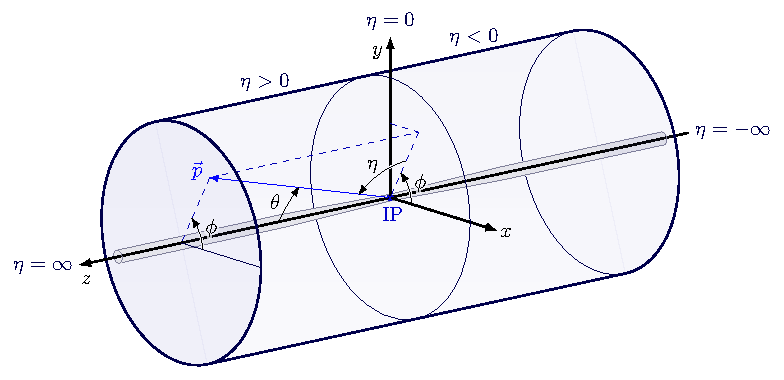
\includegraphics[width=\figwidth]{coordinate_system.pdf}
    \caption[Sketch of the CERN accelerator complex]{Sketch of the LHC ring along with the machines in the CERN accelerator complex\cite{Haffner:1621894}.}%
    \label{fig:coordinatesys}
\end{figure}

\subsection{The Inner Detector}
The closest sub detector system from the beam pipe is the Inner Detector (ID). It has a cylindircal barrel region covering $|\eta|<1$ and two end-cap regions covering 
$1 \leq \eta \leq 2.5$~\cite{BARBERIS2000331}. The ID comprises of the Pixel Detector, Semiconductor Tracker (SCT) and Transition Radiation Tracker (TRT) immersed in a 2 T solenoidal 
magnetic field. Data recorded by these components are used to reconstruct charged-particle trajectories which eventually are used to measure momenta. 

The Pixel Detector resides along the innermost radii of 33-150 mm~\cite{Aaboud_2017}. Modules of silicon pixels are arranged in three layers in the barrel region and two layers in the end-cap region. 
It gives a three-dimensional space-point reading from which primary and secondary vertices can be reconstructed. The high granularity of these pixels provide high spatial 
resolution that is beneficial in pattern recognition. The next sub component outside the ID is the Semiconductor Tracker (SCT) which consist of silicon microstrip detectors 
arranged in four barrel layers and two end-cap layers. The radii range of the SCT is 299-560 mm. The outermost sub component is the Transition Radiation Tracker (TRT) which 
is made up of gaseous straw tube detectors. It spans across 563-1066 mm radii. The straws are filled with xenon and carbon-dioxide at atmospheric pressure and each straw
has a gold-plated tungsten wire along the longitudinal axis. The transition material is a low-density foam surrounding the straws. Tracks of particles are reconstructed from TRT
data. Moreover, electron identification is also possible. A combination of measurements given by the sub components help get a high-resolution vertex and momentum measurement of
particles. 

\subsection{Calorimeters}
Detector system surrounding the ID are calorimeters. The tasks of a calorimeter include accurately measuring energies and position of incoming 
particles. The particles emerging after a certain process during collisions, interact with the active material inside the calorimeters and produce secondary particles. This process 
results into a shower of particles which is contained inside the calorimeter and recorded for accurate energy measurements. Besides good area coverage, 
sufficient depth is also an important parameter for calorimeters. In order to contain the showers, calorimeters at ATLAS are designed such that they cover a 
full $\phi$-range and $|\eta|<4.9$.  

The electromagnetic calorimeter (ECAL) is a lead-liquid-argon calorimeter split into a barrel component ($|\eta|<1.475$) and two end-cap components 
($1.375 < |\eta| < 3.2$)~\cite{TheATLASCollaboration_2008}. Over the precision physics $\eta$ region, essentially the region coinciding with the inner detector, contains highly granular
detectors which are capable of accurately measuring electron energies. The ones outside this range are coarser but still adequate for jets and missing transverse energy measurements.
The ECAL is sampling detector in which the liquid argon (active material) and lead absorbers are placed alternatively in an accordian geometry. This geometry allows for a full 
$\phi$-coverage. The incoming particles encounter the absorber, this produces charged particles which ionise the argon atoms. The resulting electrons travel towards the electrodes and 
signal is recorded. The depth of ECAL is decided as per the radiation length. The radiation length $X_0$ is a characteristic of a material which is defined as 
the length at which the energy of a particle traversing the material, is reduced by a factor of $1/e$. The thickness of ECAL is $> 22 X_0$ in the barrel and $> 26 X_0$ in the end-cap
regions. The energy resolution of the ECAL is $\sigma_E/E = 10\%/\sqrt{E} \oplus 0.7\%$~\cite{CERN-LHCC-2017-018}.

The hadronic calorimeter (HCAL) 


\subsection{Muon spectrometers}
The muon spectrometers play the significant role in accurate measurement of high energy muons. The structure is made up of three superconducting toroids, 
precision tracking chambers and trigger system. The Barrel toroid is made of eight superconducting coils, having a coil area of $5 \times 26 \text{m}^2$ each 
providing a magnetic field in the range of 0.5 to 2 T. In the end-cap region eight superconducting coils are situated inside an insulation vessel, providing magnetic 
field in the range 1 to 2 T~\cite{Palestini:2003noa}. 

The hunting of muon candidates from the collided particles is done by the ATLAS muon trigger. It comprises of the Level-1 muon trigger and the High-Level muon trigger implemented with 
different detectors. The Resistive Plate Chambers (RPCs) are placed in the Barrel region and the Thin Gap Chambers (TGCs) are placed in the End-Cap region. Different types of 
detectors are used in Barrel and End-Cap because the muon flux encountered by these regions is different. The RPCs and TGCs form the Level-1 muon trigger, it selects muon
candidates with high $p_T$ by reconstructing tracks that point directly towards the interaction point. The precision tracking 
chambers house the Monitored Drift Tubes (MDT) that perfrom the precision measurement of muon momentum. Each chamber
contains two layers, each formed by three or four layers of drift tubes. The drift tubes are made up of aluminium and are filled with $\text{Ar}-\text{CO}_2$ gas mixture.
The MDTs along with Cathode Strip Chambers (CSCs) form the High-Level muon trigger. In Run-2, for high-$p_T$ the threshold was 20 GeV for Level-1 muon trigger and 26 GeV 
for High-Level muon trigger.  


